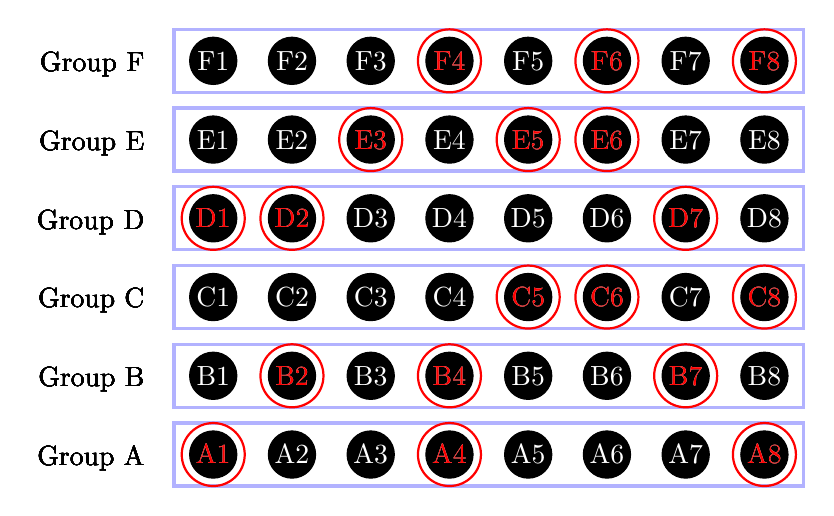
\begin{tikzpicture}
    \edef\gnames{{"A","B","C","D","E","F"}};
    \foreach \grp in {1,2,...,6} {
        \pgfmathsetmacro\gname{\gnames[\grp-1]};
        \foreach \num in {1,2,...,8} {
            \draw[blue!30!white,very thick] (-0.5,{\grp-0.4}) rectangle (7.5,{\grp+0.4});
            \node[left] at (-0.75,{\grp-0.05}) {Group \gname};
            \draw[fill=black] ({\num-1},\grp) circle (0.3) node[white] (\num) {\gname\num};
        }    
    }
    \edef\sample{{
        {1,4,8},
        {2,4,7},
        {5,6,8},
        {1,2,7},
        {3,5,6},
        {4,6,8}
    }}
    \foreach \grp in {1,2,...,6} {
        \pgfmathsetmacro\gname{\gnames[\grp-1]};
        \foreach \i in {1,2,3} {
            \pgfmathsetmacro\num{\sample[\grp-1][\i-1]};
            \draw[draw=red,thick] ({\num-1},\grp) circle (0.4) node[red] {\gname\num};
        }
    }
\end{tikzpicture}